\documentclass[border=2pt,tikz]{standalone}
\usepackage{tikz}
\usepackage{amsmath}
\usepackage{amssymb}

\begin{document}

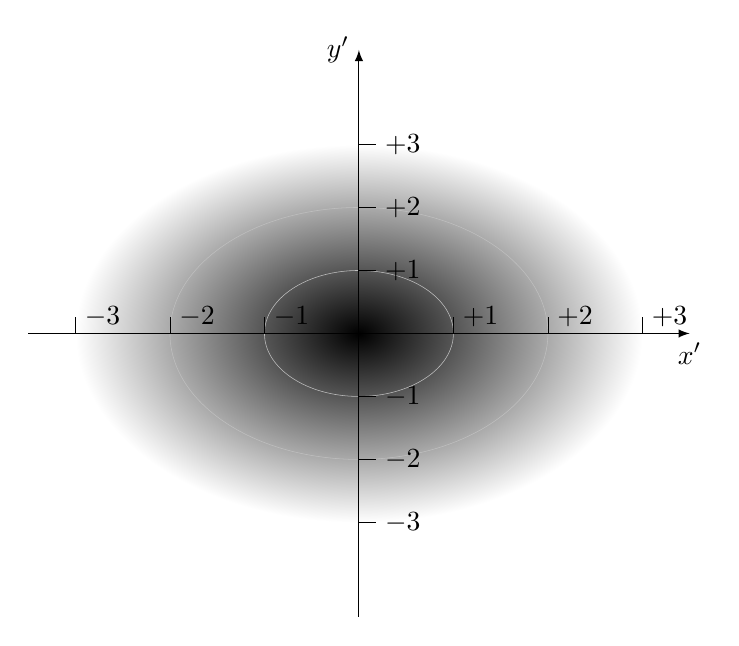
\begin{tikzpicture}[scale=3]

% FIXME: 程序有BUG,旋转之后灰度边缘不对。
\draw [very thin, lightgray!0, inner color=black!100, outer color=black!0] (0,0) ellipse (1.2 and 0.8);
\draw [very thin, lightgray] (0,0) ellipse (1.2/3*2 and 0.8/3*2); % \sigma = +-2
\draw [very thin, lightgray] (0,0) ellipse (1.2/3   and 0.8/3  ); % \sigma = +-1

% Draw x and y axis lines
\draw [->,>=latex] (-1.4,0) -- (1.4,0) node [below] {$x^\prime$};
\draw [->,>=latex] (0,-1.2) -- (0,1.2) node [left]  {$y^\prime$};

% 画标尺
\draw [very thin] ( 1.2    , 0) -- ( 1.2    , 2pt) node [right]  {$+3$};
\draw [very thin] (-1.2    , 0) -- (-1.2    , 2pt) node [right]  {$-3$};
\draw [very thin] ( 1.2/3*2, 0) -- ( 1.2/3*2, 2pt) node [right]  {$+2$};
\draw [very thin] (-1.2/3*2, 0) -- (-1.2/3*2, 2pt) node [right]  {$-2$};
\draw [very thin] ( 1.2/3  , 0) -- ( 1.2/3  , 2pt) node [right]  {$+1$};
\draw [very thin] (-1.2/3  , 0) -- (-1.2/3  , 2pt) node [right]  {$-1$};

\draw [very thin] ( 0, 0.8    ) -- ( 2pt, 0.8    ) node [right]  {$+3$};
\draw [very thin] ( 0,-0.8    ) -- ( 2pt,-0.8    ) node [right]  {$-3$};
\draw [very thin] ( 0, 0.8/3*2) -- ( 2pt, 0.8/3*2) node [right]  {$+2$};
\draw [very thin] ( 0,-0.8/3*2) -- ( 2pt,-0.8/3*2) node [right]  {$-2$};
\draw [very thin] ( 0, 0.8/3  ) -- ( 2pt, 0.8/3  ) node [right]  {$+1$};
\draw [very thin] ( 0,-0.8/3  ) -- ( 2pt,-0.8/3  ) node [right]  {$-1$};

\end{tikzpicture}

\end{document}

